\documentclass[12pt,letterpaper]{hmcpset}
\usepackage[margin=1in]{geometry}
\usepackage{graphicx}
\usepackage{amsmath,amssymb}
\usepackage{enumerate}

\newcommand{\dg}[1]{\ensuremath{#1^o}}

% info for header block in upper right hand corner
\name{Evan Hubinger}
\class{Physics 24A - Section 1}
\assignment{Dynamical Systems}
\duedate{Monday, April 4, 2016}

\begin{document}

\problemlist{7.\{17, 20, 28, 34, 37\}}



\begin{problem}[Rod and springs - KK 7.17]
A rod of length $l$ and mass $m$, pivoted at one end, is held by a spring at
its midpoint and a spring at its far end, both pulling in opposite
directions. The springs have spring constant $k$, and at equilibrium their
pull is perpendicular to the rod. Find the frequency of small oscillations
around the equilibrium position. (Don't forget about gravity.)
\begin{center}
    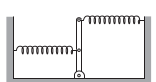
\includegraphics{img/7_17}
\end{center}
\end{problem}
\begin{solution}
    \vfill
\end{solution}
\clearpage

\begin{problem}[Falling plank - KK 7.20]
A thick plank of mass $M$ and length $l$ is pivoted at one end, as shown. The
plank is released at $\dg{60}$ from the vertical. What is the magnitude and
direction of the force on the pivot when the plank is horizontal?
\begin{center}
    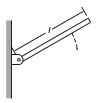
\includegraphics{img/7_20}
\end{center}
\end{problem}
\begin{solution}
    \vfill
\end{solution}
\clearpage

\begin{problem}[Yo-yo pulled at angle - KK 7.28]
The yo-yo of the previous problem is pulled so that the string makes an angle
$\theta$ with the horizontal. For what value of $\theta$ does the yo-yo have
no tendency to rotate?
\begin{center}
    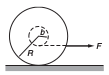
\includegraphics{img/7_28}
\end{center}
\end{problem}
\begin{solution}
    \vfill
\end{solution}
\clearpage

\begin{problem}[Marble in dish* - KK 7.34]
A marble of radius $b$ rolls back and forth in a shallow dish of radius $R$,
where $R \gg b$. Find the frequency of small oscillations.
\end{problem}
\begin{solution}
    \vfill
\end{solution}
\clearpage

\begin{problem}[Plank and ball* - KK 7.37]
\begin{enumerate}[(a)]
\item A plank of length $2l$ and mass $M$ lies on a frictionless table. A
ball of mass $m$ and speed $v_{0}$ strikes its end as shown. Find the final
velocity of the ball, $v_{\rm f}$, assuming that mechanical energy is
conserved and that $v_{\rm f}$ is along the original line of motion.
\item Find $v_{\rm f}$ assuming that the stick is pivoted at the lower end.
\end{enumerate}
\begin{center}
    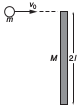
\includegraphics{img/7_37}
\end{center}
\end{problem}
\begin{solution}
    \vfill
\end{solution}
\clearpage

\end{document}
